\documentclass[11pt,a4paper]{article}
\usepackage[margin=1in]{geometry}
\usepackage{amsmath,amssymb}
\usepackage{graphicx}
\usepackage{hyperref}
\usepackage[numbers,sort]{natbib}
\usepackage{booktabs}
\usepackage{caption}
\captionsetup{font=small,labelfont=bf}
\setlength{\parskip}{0.6em}
\setlength{\parindent}{0em}

\title{Fear is contagious too: behavioural feedback in epidemic spreading on networks}
\author{Ruilei Wang (24328412) \and Xuan Truong Nguyen (24012326)}
\date{CITS4403 Group Project \\ October 2026}

\begin{document}
\maketitle

\begin{abstract}
We couple a network SIR epidemic with a second contagion, risk perception,
and compare three behavioural-feedback rules head to head: local observation
of sick contacts, social imitation of cautious neighbours, and global
broadcast nudges (uniform or hub-targeted). Across 13,290 simulations on
Watts--Strogatz, Barabasi--Albert and degree-matched Erdos--Renyi networks
($N=1000$), local observation averts the most infections per unit of social
cost when averaged over the tested grid on each topology. Running to
extinction removes broadcast's apparent final-size advantage on
Watts--Strogatz networks. Degree-aware contact costs remove most of hub
targeting's efficiency advantage, while intermediate fear decay produces
repeated prevalence peaks under broadcast. These are comparative findings
within synthetic networks, not calibrated intervention recommendations.
\end{abstract}

\section{Introduction}
Epidemics spread over contact networks, but so does fear of infection, and
fear changes contacts \cite{Funk2010}. Classical compartmental models
\cite{Kermack1927} and their network extensions \cite{Newman2002} usually
treat behaviour as fixed, even though real responses (avoiding contacts,
masking, staying home) feed back on transmission. Our research question is:
which behavioural-feedback rule minimises epidemic final size \emph{per unit
of social cost}, measured as contacts forgone? We test three candidate
theories in one framework: (i)~imitating neighbours' precautions, (ii)~local
observation of sick contacts, and (iii)~broadcast nudges triggered at a
prevalence threshold.

Our proposal stated three hypotheses:
\begin{itemize}
\item \textbf{H1:} intermediate fear-memory decay produces multi-wave
dynamics.
\item \textbf{H2:} on scale-free networks hub-targeted nudges dominate,
while on homogeneous networks they do not.
\item \textbf{H3:} imitation-based behaviour amplifies and overshoots,
producing oscillations.
\end{itemize} Coupled awareness and disease models already show that local
protective responses can reduce epidemic spread \cite{Funk2009}. Our
contribution is a controlled comparison of three response rules on the same
epidemic engine and three topologies, with explicit contact-cost accounting.
We investigate how memory and targeting affect this comparison; the
hub-pool ceiling is an imposed policy constraint, not a new network law.

\section{Model}
Each node carries a disease state $S$, $I$ or $R$ and a fear level
$f \in [0,1]$. A node is \emph{cautious} when $f > \theta$ with $\theta=0.5$.
Updates are synchronous with fixed parameters $N=1000$, per-edge
transmission probability $\beta=0.12$, recovery probability $\gamma=0.05$,
caution effectiveness $q=0.8$, broadcast trigger prevalence $0.02$, hub pool
$10\%$ by degree, and 10 initially infected nodes. Topologies are
Watts--Strogatz (WS, $k=6$, rewiring $0.1$), Barabasi--Albert (BA, $m=3$)
\cite{Watts1998,Barabasi1999}, and Erdos--Renyi (ER) with $p=6/(n-1)$ so the
expected mean degree matches at $6$.

\paragraph{Fear updates.} Let $I_j$ indicate infected neighbours of $i$,
$C_i$ the cautious-neighbour fraction and $\hat{I}_i$ the
infected-neighbour fraction. Observation adds fear from sick contacts and
forgets geometrically:
$f_i \leftarrow f_i + \alpha \hat{I}_i - \delta f_i$.
Imitation copies caution while retaining a local risk cue, with $2\%$
innovators seeded cautious so copying has something to amplify:
$f_i \leftarrow f_i + \alpha(C_i - f_i) + \alpha \hat{I}_i$, then multiplied
by $(1-\delta/2)$. Thus imitation has slower effective forgetting at the
same nominal $\delta$; this is a modelling assumption, not a matched-memory
comparison. Cautious flags are initialised from the seeded fear levels, and
$C_i$ uses the previous step's flags. Broadcast decays fear by $(1-\delta)$ and, when prevalence
reaches $0.02$, sets fear to $1$ for compliers, each included with probability
$p_{\text{comply}}$ (uniform) or, for hub targeting, restricted to the top
degree decile with probability $\min(1, \text{budget}/0.1)$ so budgets up to
$10\%$ reach equal expected node counts per triggered update under both
policies. Uniform sampling can reach new nodes on successive updates, whereas
the hub policy repeatedly samples its fixed pool. Here $\alpha$ is
coupling strength for local rules and the compliance budget for broadcast,
and $\delta$ is fear-memory decay. All fears are clipped to $[0,1]$.

\paragraph{Disease updates.} A susceptible node with $c_1$ non-cautious and
$c_2$ cautious infected neighbours escapes with probability $e_1^{c_1}
e_2^{c_2}$, where $e_1 = 1-\beta(1-qc_i)$ and
$e_2 = 1-\beta(1-q)(1-qc_i)$ with $c_i \in \{0,1\}$ its own caution state, so
caution protects both ways. Recovery and infection both use the disease
state at the start of a step, so an infector can transmit and recover during
the same update. Infected nodes recover with probability $\gamma$.
Outcomes are final size (fraction ever infected), peak prevalence, duration,
detected wave count (peak detection with prominence $\max(0.01, 0.2 \times
\text{peak})$ and at least 10 steps separation), oscillation index, and social
cost. Our primary degree-aware cost is
$K_D=(q/2)\sum_t\sum_i c_i(t)k_i$; the original mean-degree proxy
$K_M=(q\bar{k}/2)\sum_t\sum_i c_i(t)$ is retained for sensitivity analysis.
Here $c_i(t)$ is the caution applied during that step's transmission.
These are protective-effort proxies in edge-steps: adjacency is fixed, edges
are not deleted, and steps are not calibrated to days. The $1/2$ factor is
an endpoint-accounting convention, not an exact count of removed edges.
Costs end at disease extinction and exclude any later residual caution.
Efficiency is $N(F_0-F)/K$, infections averted per edge-step, with a
negligible denominator offset of one edge-step to handle zero cost.
Runs stop at extinction, with a 5,000-step safety limit; unfinished runs are
flagged and cannot supply a final size to the experiment pipeline.
The homogeneous ODE is a reference approximation, not an exact validation
target for a clustered, discrete-time network.

\section{Experimental design}
Three regenerated grids total 13,290 configurations: a full
topology$\times$rule$\times\alpha\times\delta$ pilot ($9{,}090$ runs, 30
seeds), an equal-budget hub-versus-uniform zoom ($3{,}600$ runs, 30 seeds),
and a transmission sweep over $\beta \in \{0.03,0.06,0.09,0.12,0.2\}$
($600$ runs, 20 seeds), plus 80 WS runs against a homogeneous SIR ordinary
differential equation. Measures, seeds, and the no-behaviour baseline are
fixed across comparisons. The pilot uses
$\alpha\in\{0,0.25,0.5,0.75,1\}$ and
$\delta\in\{0,0.05,0.15,0.3,0.6\}$; the zoom uses budgets
$\{0.02,0.05,0.08,0.10,0.15\}$ and $\delta\in\{0,0.05,0.15,0.3\}$.
Seeds are $0$--$29$, or $0$--$19$ for transmission and ODE comparisons.
The transmission comparison fixes observation at $\alpha=0.75$, $\delta=0.10$.
Means aggregate 600 runs per positive-coupling tradeoff point and 120 per
hub-budget point. Efficiency intervals use 2,000 paired bootstrap resamples
of seed clusters, preserving each seed's baseline and parameter cells;
transmission and ODE error bars show sample SD across 20 seeds.
Boundary checks cover zero transmission, immediate recovery when
$\gamma=1$ and $\beta=0$, zero initial infections, determinism, and the
no-behaviour limit. Regression tests cover termination flags, cost timing,
innovator initialisation, degree accounting, sparse/dense trajectory
equivalence, and full-configuration caching. Cache identities include every
simulation parameter and a fingerprint of the model source.
\texttt{python -m src.run\_sweeps --workers 4} regenerates all grids;
\texttt{notebooks/04\_analysis.ipynb} regenerates the figures and summaries.
\texttt{data/} holds the corrected CSVs and provenance; earlier outputs are
retained as legacy data and are not used in the analysis:
\url{https://github.com/idawang142/4403PROJECT}.

\section{Results}
\paragraph{Observation has the highest grid-average efficiency.}
Under degree-aware accounting, observation averts $0.00498$ infections per
edge-step on WS (95\% bootstrap interval $0.00478$--$0.00519$), $0.00236$
on BA ($0.00229$--$0.00243$), and $0.00209$ on ER
($0.00200$--$0.00218$; Fig.~\ref{fig:tradeoff}, Table~\ref{tab:eff}).
It also leads under the mean-degree proxy. This is a ratio of grid-average
benefit to cost, not a claim that observation wins every parameter cell.
On WS, observation's mean final size is $0.603$ versus $0.642$ for uniform
broadcast, which costs $848{,}000$ versus $80{,}000$ edge-steps, about
$10.6$ times as much. Uniform broadcast has smaller grid-average epidemics
on BA and ER, but higher costs. All runs reach extinction; the longest lasts
$1{,}197$ steps. The earlier 500-step cutoff had made broadcast look more
effective by excluding later infections and protective effort.

\begin{table}[htbp]
\centering
\caption{Grid-average outcomes at extinction (600 runs per row).
Cost is the degree-aware proxy in edge-steps; efficiency is infections
averted per edge-step, shown in units of $10^{-3}$.}
\label{tab:eff}
{\small
\begin{tabular}{llccc}
\toprule
Topology & Rule & Final size & Degree-aware cost & Efficiency ($\times10^{-3}$) \\
\midrule
WS & observation & 0.603 & 79,696 & 4.98 \\
BA & observation & 0.660 & 140,227 & 2.36 \\
ER & observation & 0.695 & 140,046 & 2.09 \\
WS & imitation & 0.657 & 251,777 & 1.36 \\
BA & imitation & 0.651 & 308,351 & 1.10 \\
ER & imitation & 0.687 & 331,507 & 0.91 \\
BA & broadcast & 0.586 & 635,082 & 0.64 \\
BA & broadcast\_hub & 0.944 & 93,962 & 0.50 \\
WS & broadcast & 0.642 & 847,806 & 0.42 \\
WS & broadcast\_hub & 0.985 & 34,700 & 0.42 \\
ER & broadcast & 0.666 & 828,287 & 0.39 \\
ER & broadcast\_hub & 0.977 & 45,064 & 0.24 \\
\bottomrule
\end{tabular}}
\end{table}

\paragraph{Memory governs regimes; broadcast chatters (H1 reframed).}
Final size under full observation coupling rises from $0.073$ at $\delta=0$
to $0.961$ at $\delta=0.6$ on WS (Fig.~\ref{fig:phase}): memory, not just
responsiveness, protects. Broadcast shows the sharpest regime change: with
perfect memory ($\delta=0$) prevalence is held down in about one wave, while
small positive decay ($\delta=0.05$) lets protection lapse and reignite,
averaging $19.10$ detected peaks with a maximum of $35$ over the
positive-compliance grid, compared with $1.04$ at zero decay. The largest
mean peak count occurs at $\delta=0.05$, supporting H1 for this broadcast
grid. These algorithmic peaks need not be independent outbreaks, and this
finite sweep does not establish a phase transition.

\paragraph{Hub efficiency depends on contact accounting (H2 not general).}
The mean-degree proxy gives hub targeting higher BA efficiency at every
tested budget. Degree weighting removes most of this advantage: the hub
point estimate exceeds uniform only at budget $0.02$ ($0.000330$ versus
$0.000289$); uniform is more efficient at $0.05$--$0.15$.
At $0.15$, the corresponding efficiencies are $0.000480$ for hubs and
$0.001163$ for uniform (Fig.~\ref{fig:zoom}). Thus H2 is not generally
supported by the primary cost measure. Hub final size plateaus near $0.944$
from budget $0.10$, while uniform improves from $0.809$ to $0.723$.
The plateau follows the imposed pool cap; above $10\%$, per-trigger coverage
is no longer equal. Targeting has smaller raw effects on WS and ER under
this policy, rather than being intrinsically ineffective on those networks.

\paragraph{The variability index cannot establish overshoot (H3 unresolved).}
Imitation has the highest oscillation index among the rules ($1.367$), but
the no-behaviour baseline scores higher still ($1.456$) because the index
rewards a single tall peak as well as genuine fluctuation, so H3 remains
unresolved by this metric. A fluctuation-specific measure or trajectory
analysis is needed before claiming overshoot.

\paragraph{Observation remains effective against its baseline.}
Without behaviour all topologies saturate near complete infection by
$\beta=0.09$; observation at one fixed untuned setting ($\alpha=0.75$,
$\delta=0.10$) holds WS below $0.6$ even at $\beta=0.20$, and WS is the most
suppressible topology at every tested $\beta$ (Fig.~\ref{fig:beta}). The
comparison includes no other behavioural rules, so it does not establish
their ordering across transmission rates. Against the homogeneous reference,
at $\beta=0.03$
WS infects $75.1\%$ (SD $7.5$pp) against $97.0\%$ for the ODE
(Fig.~\ref{fig:meanfield}). Clustering and discrete-time effects are
plausible contributors to this gap, but their contributions have not been
isolated; this is a reference comparison rather than proof of engine validity.

\begin{figure}[htbp]
\centering
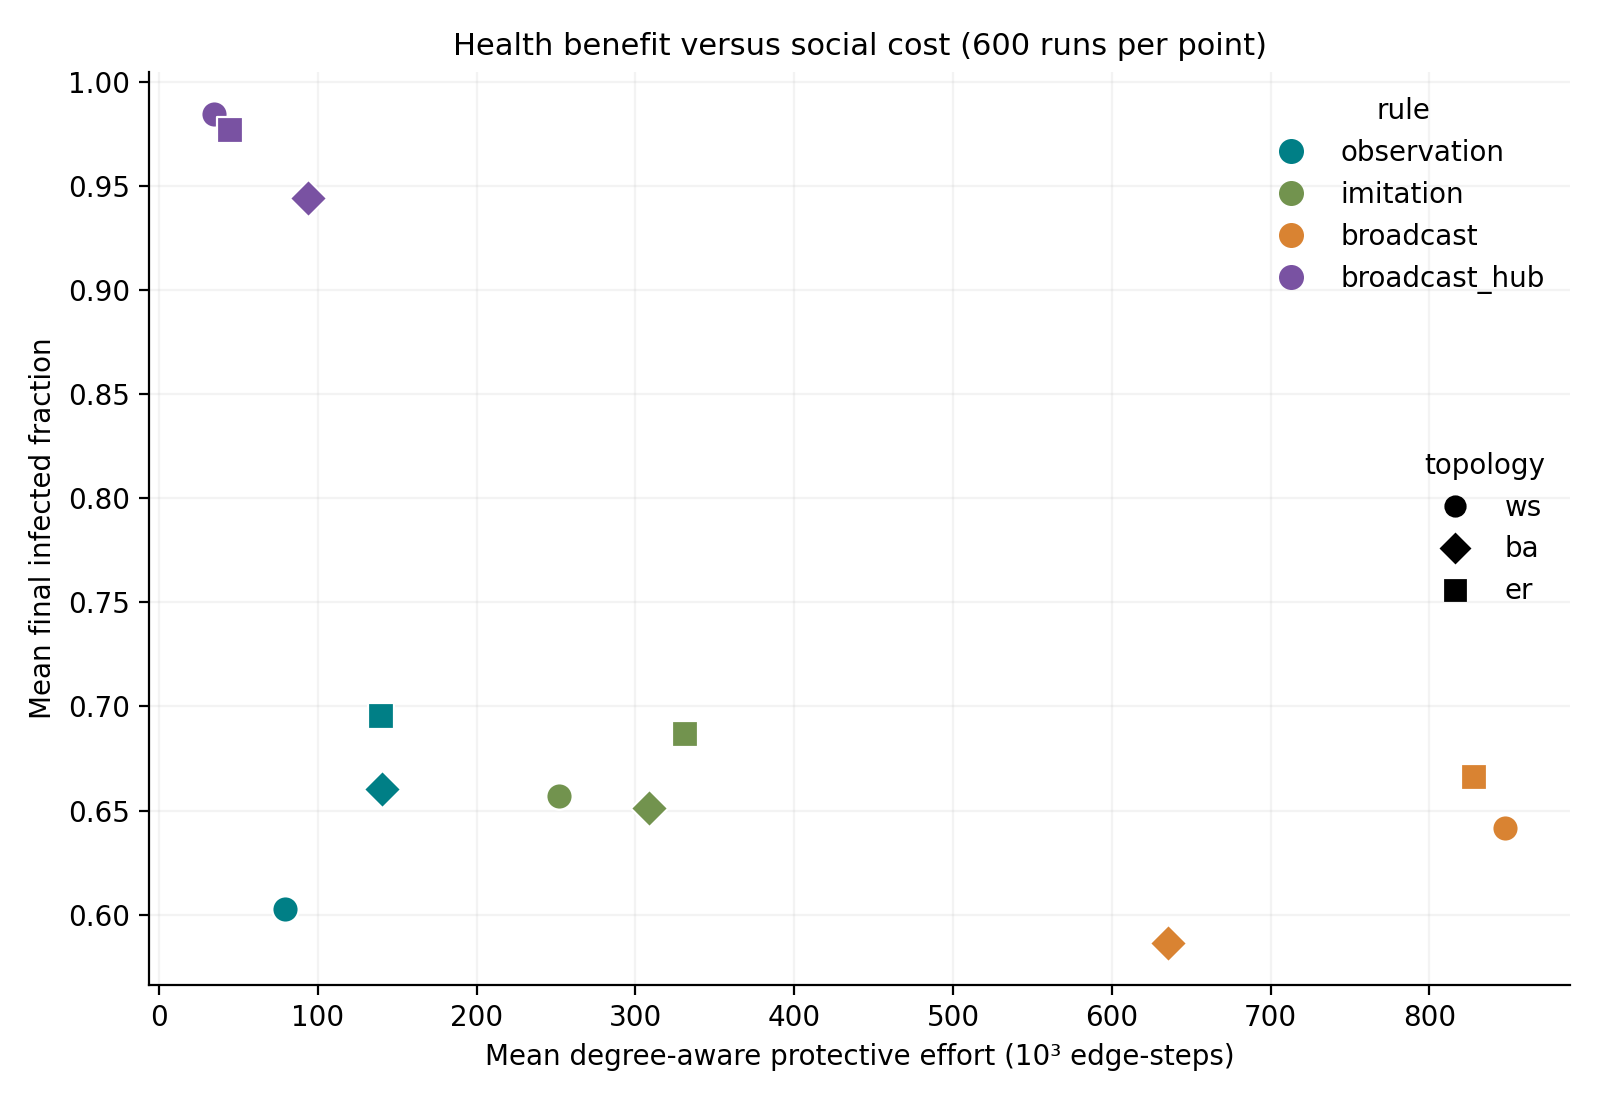
\includegraphics[width=\linewidth]{figs/tradeoff.png}
\caption{Health benefit versus social cost selects observation. Mean final
infected fraction against mean degree-aware protective effort in thousands of edge-steps;
each point averages 600 runs. Colour marks the rule, symbol the topology.
Lower and further left is better on both axes.}
\label{fig:tradeoff}
\end{figure}

\begin{figure}[htbp]
\centering
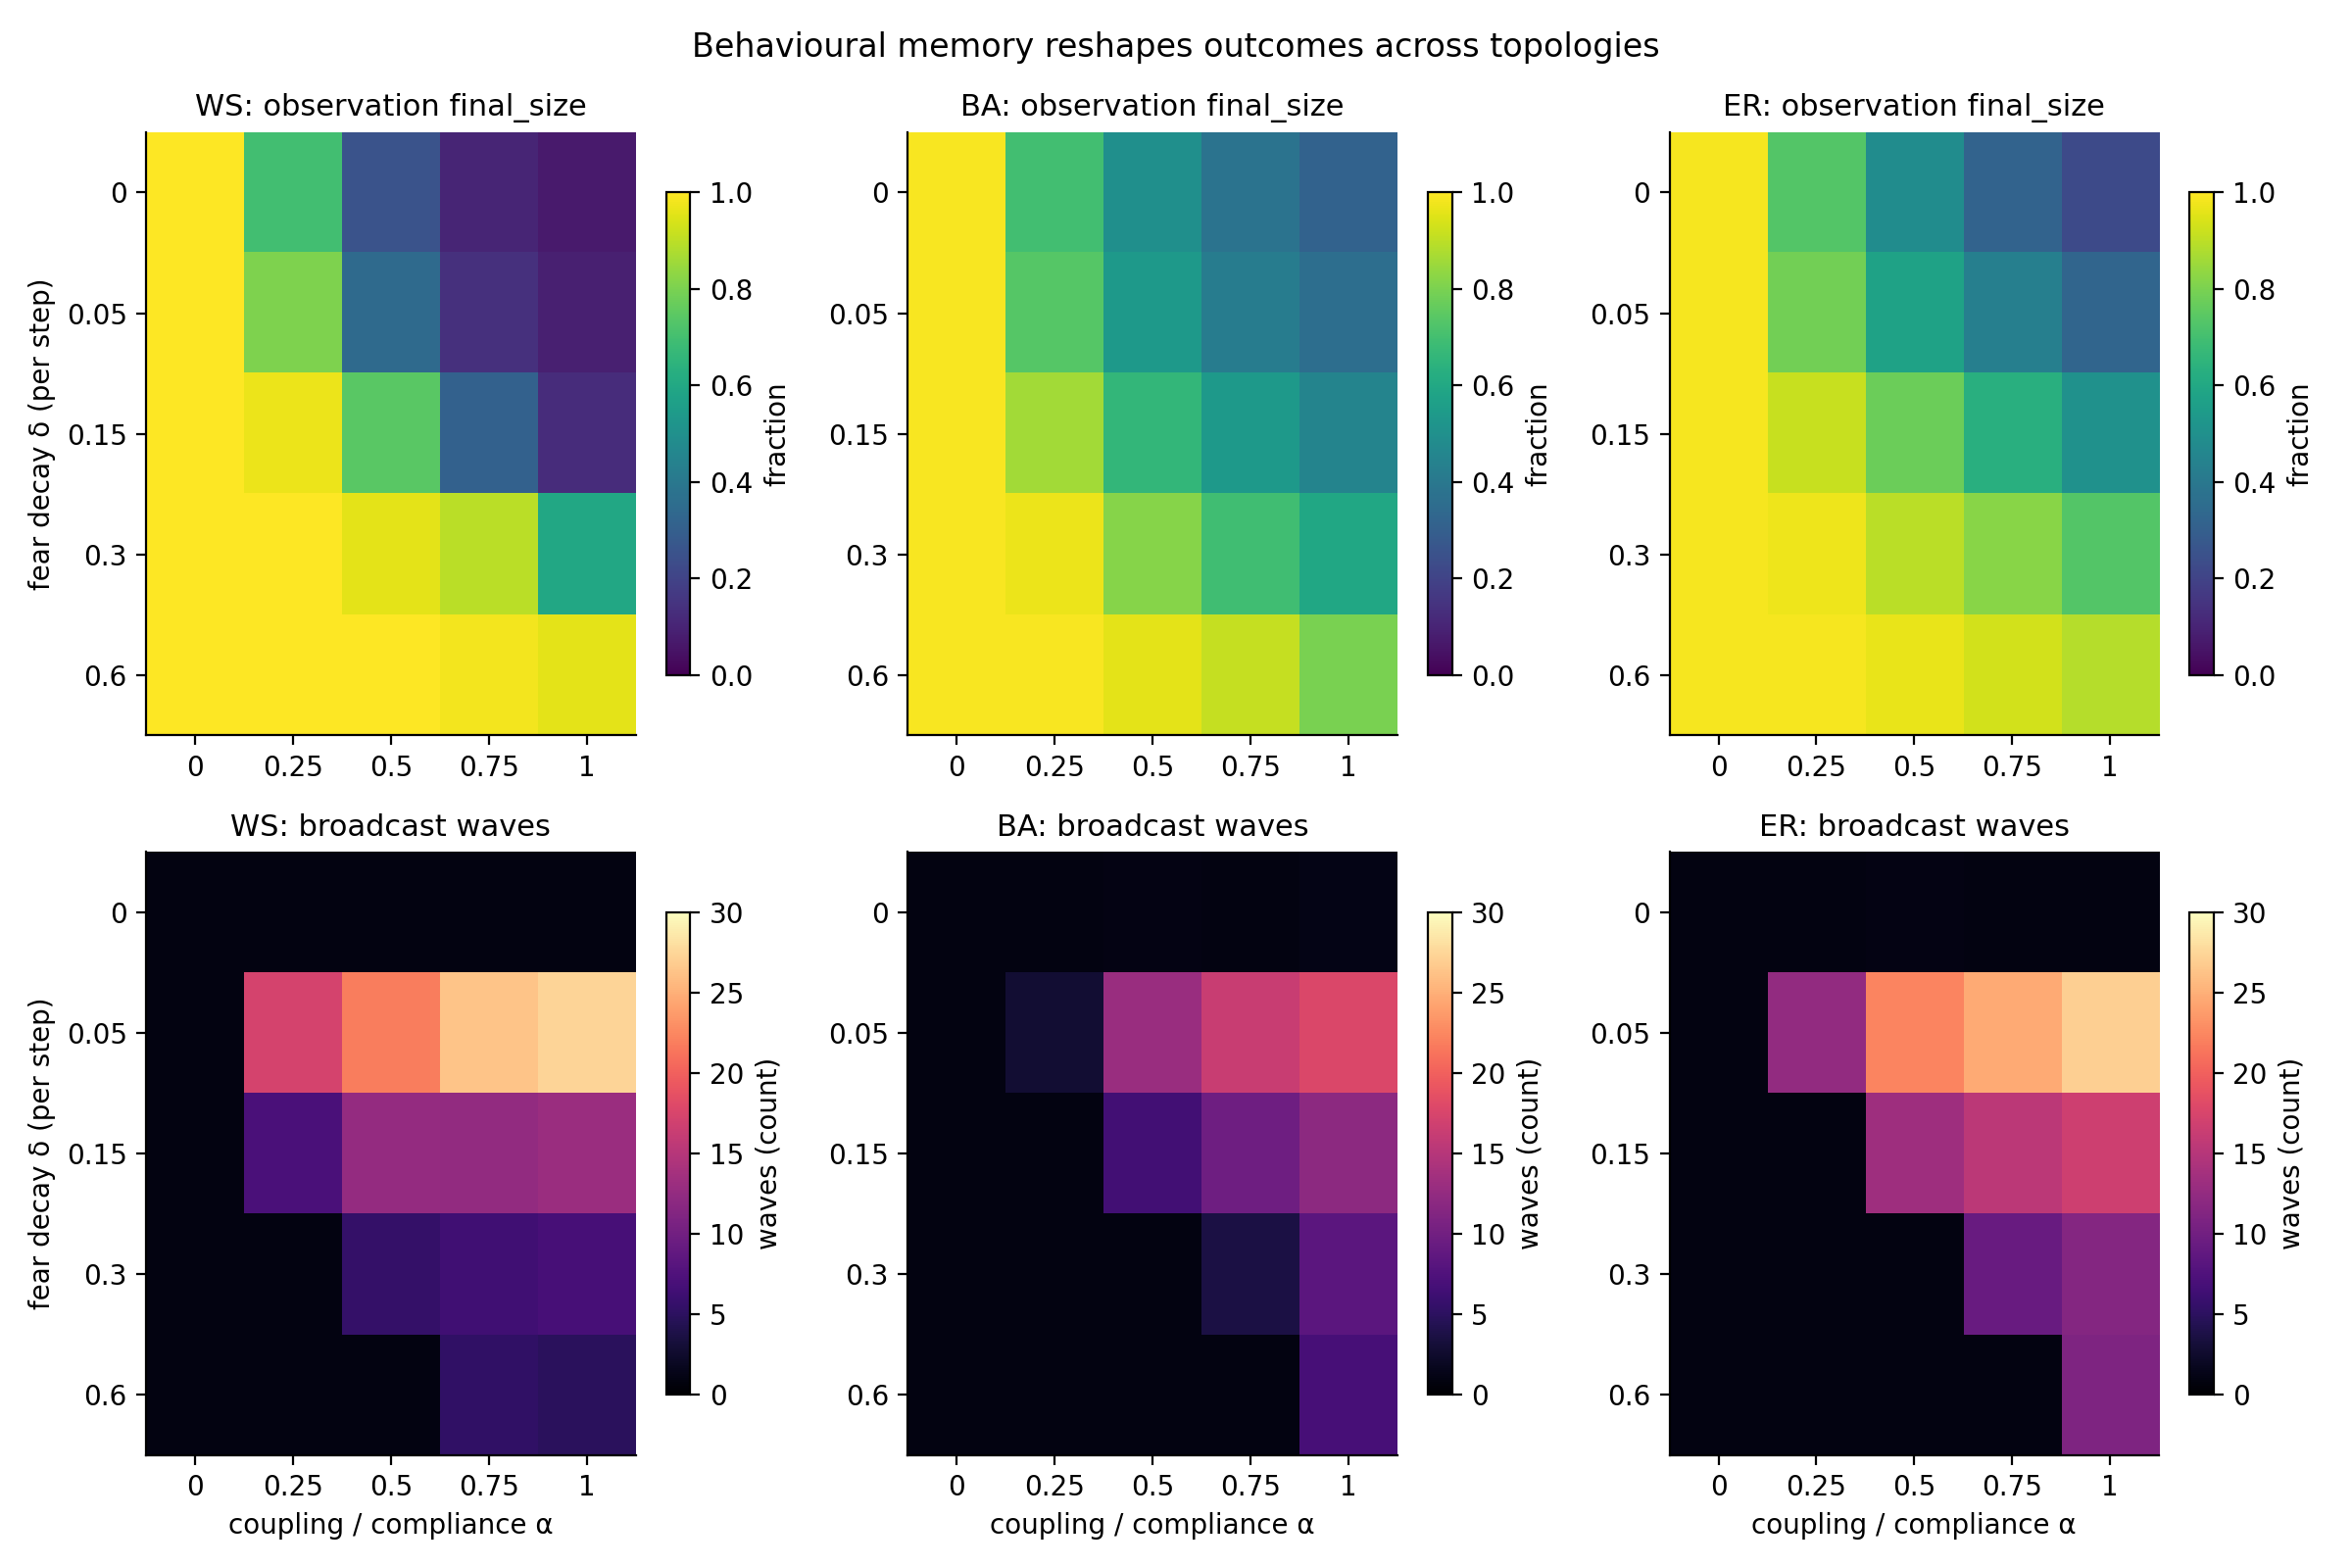
\includegraphics[width=\linewidth]{figs/phase_panels.png}
\caption{Behavioural memory reshapes outcomes. Top: mean final infected
fraction under local observation. Bottom: mean detected wave count under
global broadcast. Each cell averages 30 seeds; colour scales are fixed
across topologies within a row (fraction 0 to 1; detected peaks 0 to 30).}
\label{fig:phase}
\end{figure}

\begin{figure}[htbp]
\centering
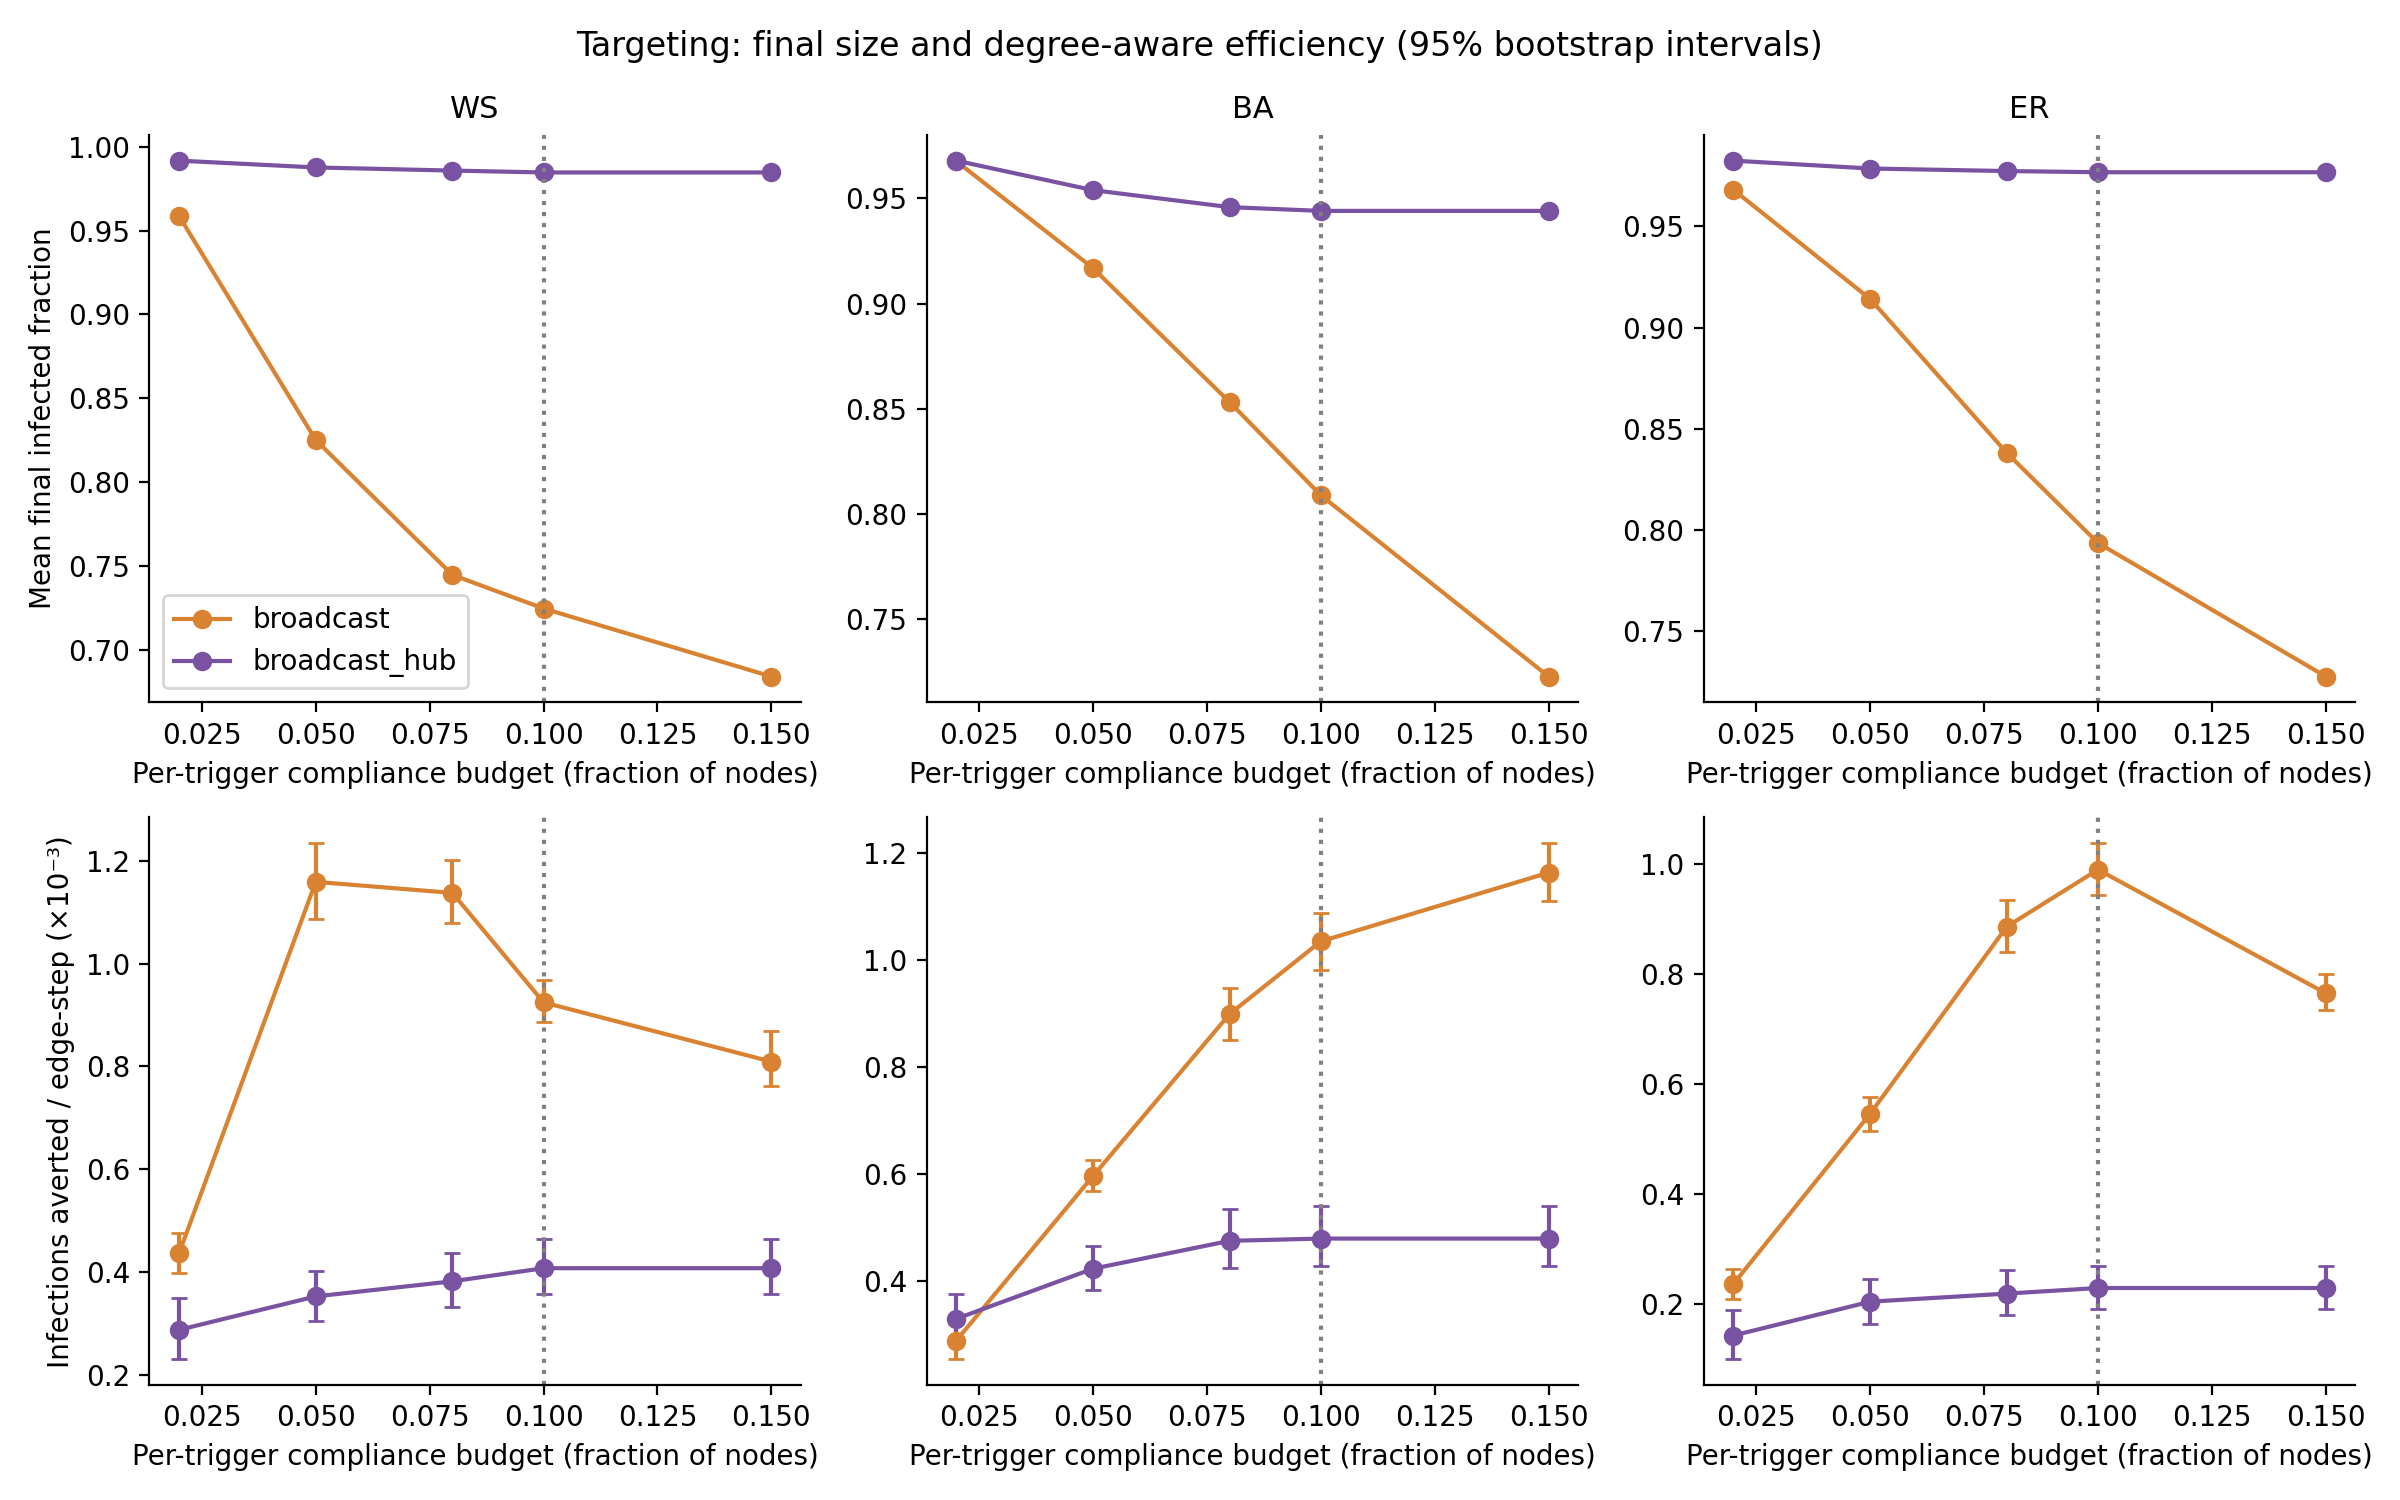
\includegraphics[width=\linewidth]{figs/zoom_h2.png}
\caption{Targeting depends on the cost measure. Top: mean final infected
fraction. Bottom: degree-aware efficiency with 95\% paired seed-bootstrap
intervals. Each point pools 120 runs; budget is the expected fraction of
recipients per triggered update. The dotted line marks the $10\%$ pool limit.}
\label{fig:zoom}
\end{figure}

\begin{figure}[htbp]
\centering
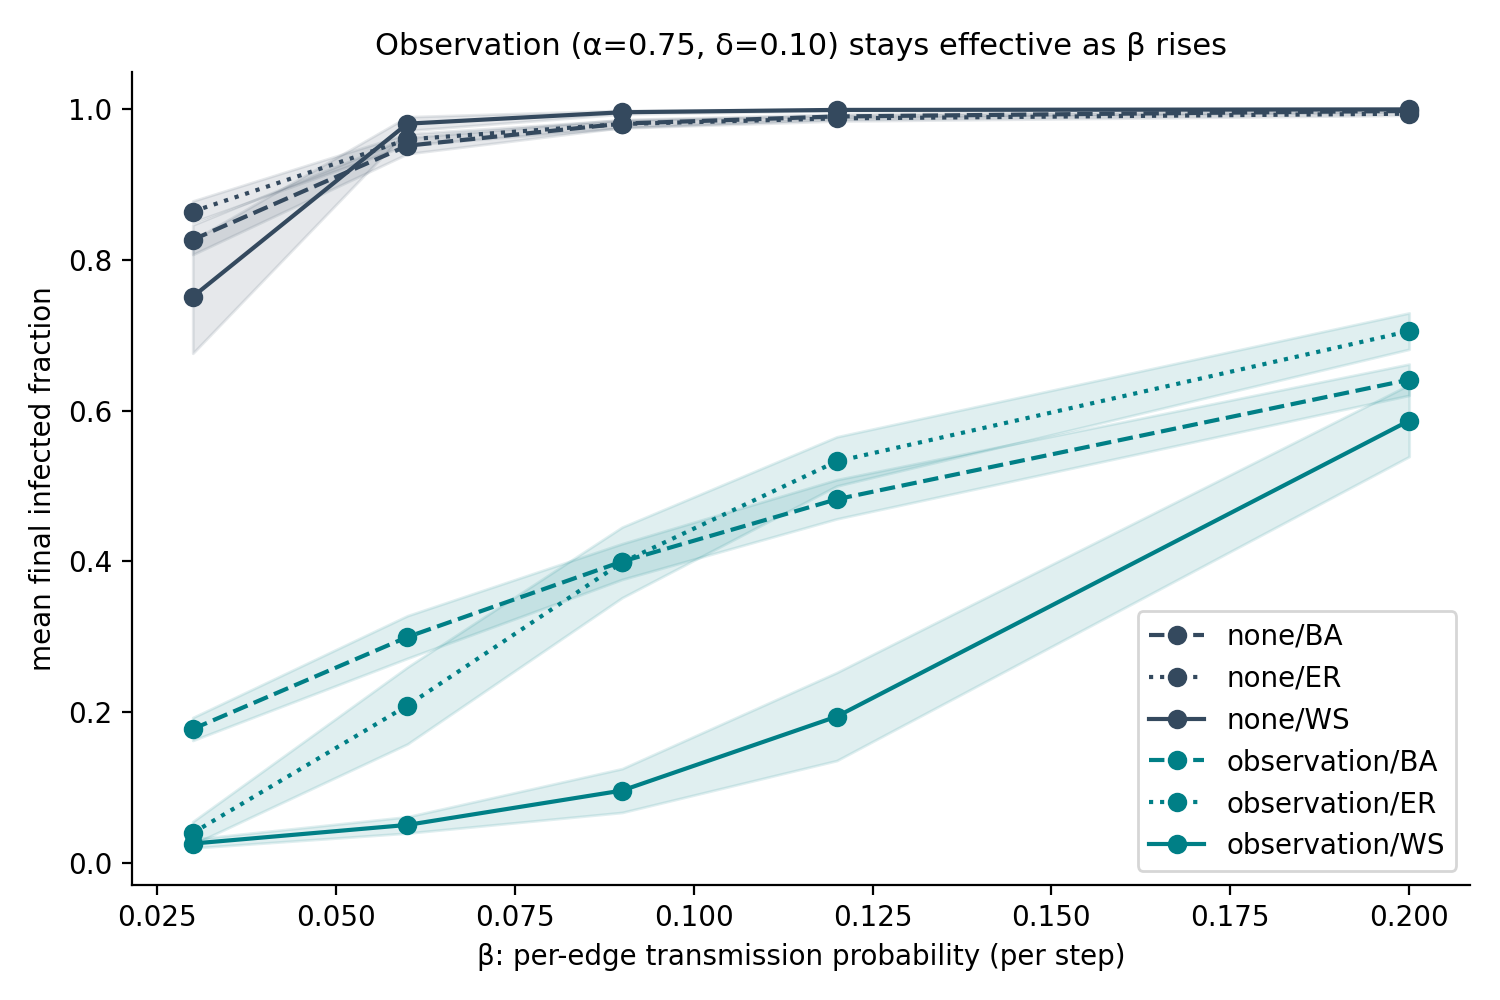
\includegraphics[width=\linewidth]{figs/beta_sweep.png}
\caption{Observation stays effective as transmission rises. Mean final
infected fraction against per-edge transmission probability per step for no
behaviour and observation ($\alpha=0.75$, $\delta=0.10$); bands show $\pm1$
sample SD across 20 seeds. Line style marks topology, colour marks rule.}
\label{fig:beta}
\end{figure}

\begin{figure}[htbp]
\centering
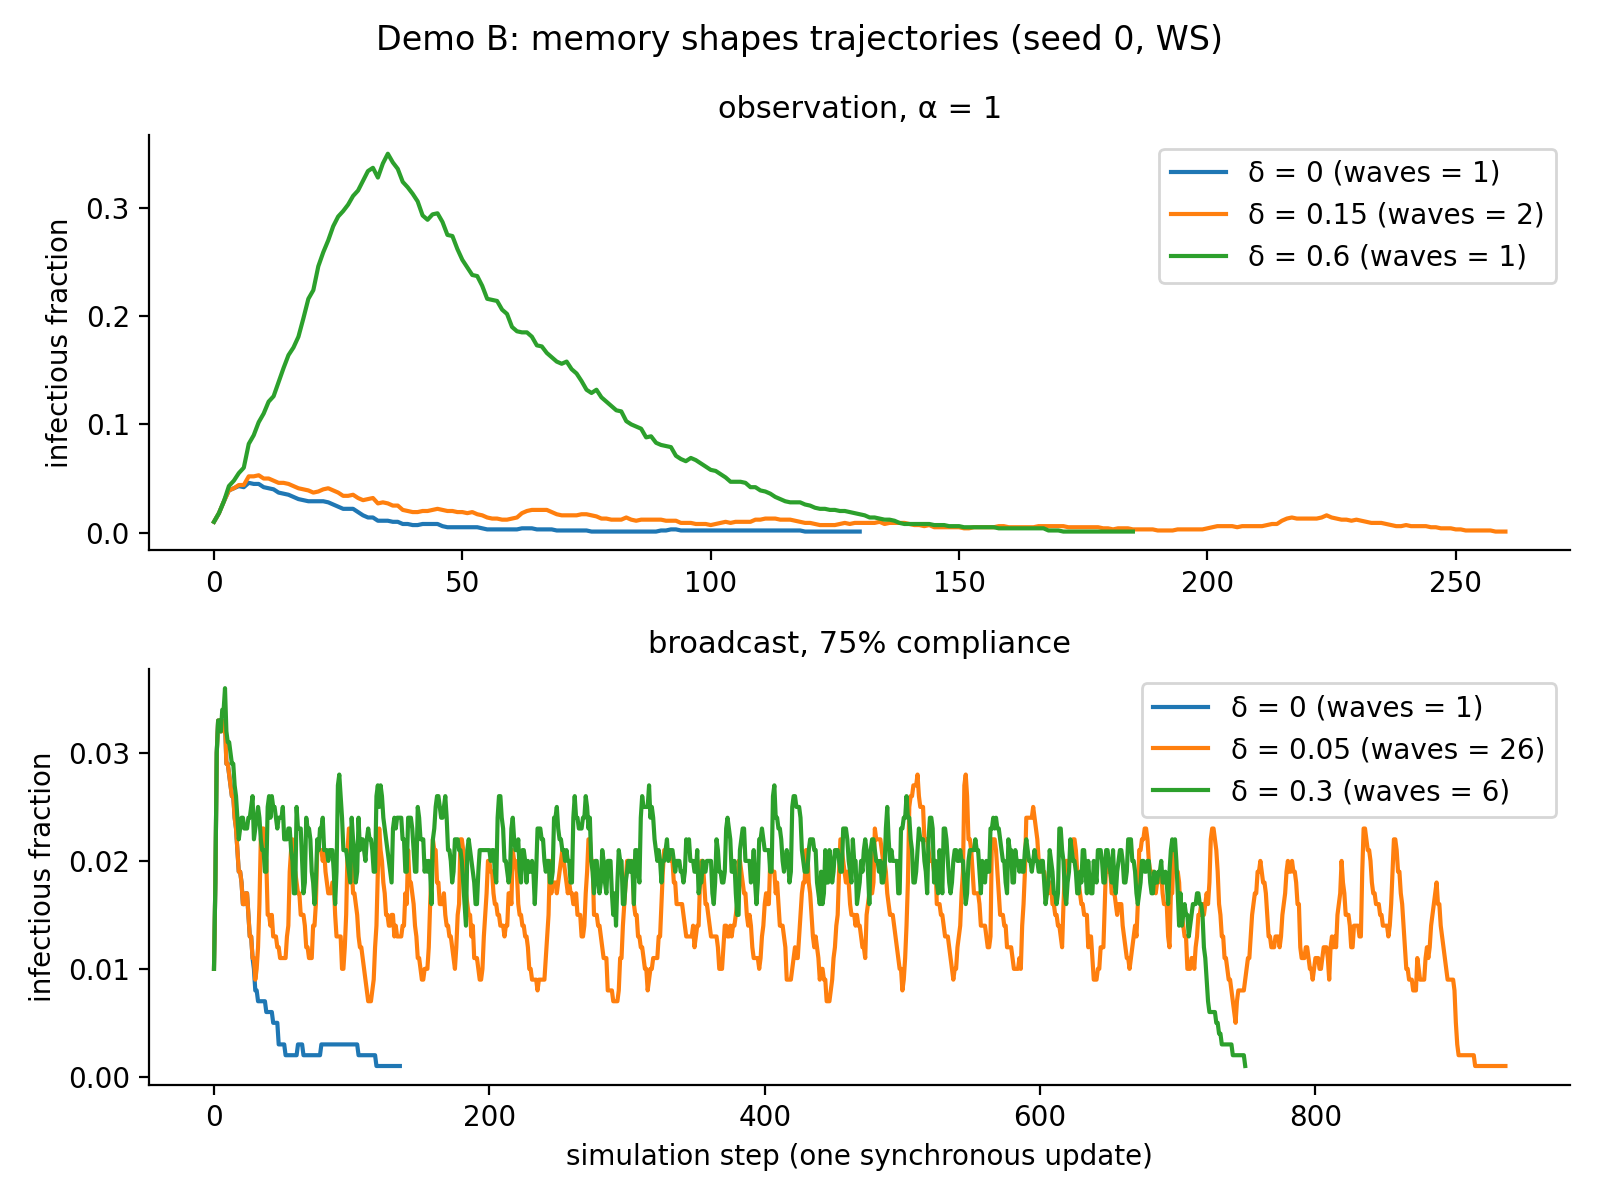
\includegraphics[width=\linewidth]{figs/timeseries.png}
\caption{Memory shapes trajectories. Infectious fraction against simulation
step for single WS runs (seed 0): local observation at full coupling (top)
and $75\%$-compliance broadcast with trigger $0.02$ (bottom) across fear
decay rates. Every illustrated run ends at extinction.}
\label{fig:timeseries}
\end{figure}

\begin{figure}[htbp]
\centering
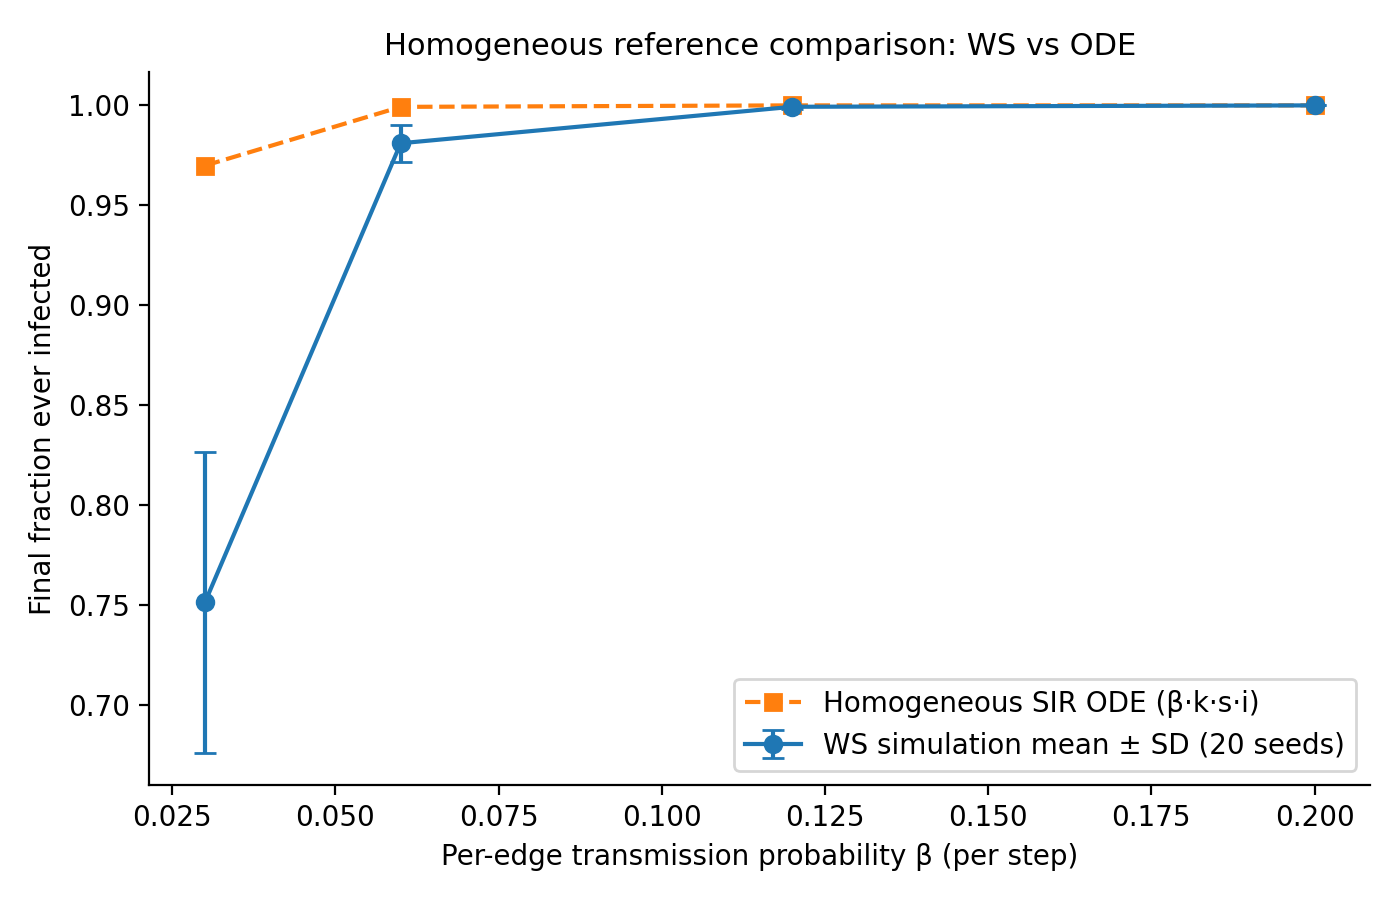
\includegraphics[width=\linewidth]{figs/mean_field.png}
\caption{Homogeneous reference comparison. WS mean final
size with sample SD (20 seeds) against the SIR ordinary differential
equation with incidence $\beta k s i$ ($k=6$) at $\gamma=0.05$. The gap at
low $\beta$ is reported without attributing it to a single mechanism.}
\label{fig:meanfield}
\end{figure}

\section{Discussion and conclusions}
\label{sec:discussion}
Local observation has the highest grid-average efficiency under both cost
proxies. A plausible explanation is that local risk links protection to
nearby infection; this mechanism has not been isolated by an ablation.
Broadcast generates repeated threshold responses and persistent infections,
making extinction-complete evaluation essential. Hub targeting illustrates
how a seemingly favourable efficiency ranking can depend on underpricing
high-degree nodes. The evidence supports a model comparison, not advice for
real populations.

All networks are synthetic, costs are endpoint-effort proxies, and residual
caution after extinction is excluded. Rankings depend on grid weights and
the cost convention. The fixed trigger and pool cap constrain interventions;
nominal decay does not match effective memory across rules. Wave counts
depend on the detector, while the variability index leaves H3 unresolved.
Bootstrap intervals capture seed variability within the fixed design, not
uncertainty in these assumptions. Useful extensions are empirical contact
networks, matched effective memory, adaptive triggers, wave-detector
sensitivity, and cost-matched policy frontiers.

\clearpage
\bibliographystyle{plainnat}
\begin{thebibliography}{6}
\bibitem[Kermack and McKendrick(1927)]{Kermack1927}
W.~O. Kermack and A.~G. McKendrick.
\newblock A contribution to the mathematical theory of epidemics.
\newblock {\em Proceedings of the Royal Society of London A}, 115(772):700--721,
  1927.
\bibitem[Watts and Strogatz(1998)]{Watts1998}
D.~J. Watts and S.~H. Strogatz.
\newblock Collective dynamics of `small-world' networks.
\newblock {\em Nature}, 393:440--442, 1998.
\bibitem[Barab\'asi and Albert(1999)]{Barabasi1999}
A.-L. Barab\'asi and R.~Albert.
\newblock Emergence of scaling in random networks.
\newblock {\em Science}, 286(5439):509--512, 1999.
\bibitem[Funk et~al.(2010)]{Funk2010}
S.~Funk, M.~Salath\'e, and V.~A.~A. Jansen.
\newblock Modelling the influence of human behaviour on the spread of
  infectious diseases: a review.
\newblock {\em Journal of the Royal Society Interface}, 7(50):1247--1256, 2010.
\bibitem[Newman(2002)]{Newman2002}
M.~E.~J. Newman.
\newblock Spread of epidemic disease on networks.
\newblock {\em Physical Review E}, 66(1):016128, 2002.
\bibitem[Funk et~al.(2009)]{Funk2009}
S.~Funk, E.~Gilad, C.~Watkins, and V.~A.~A. Jansen.
\newblock The spread of awareness and its impact on epidemic outbreaks.
\newblock {\em Proceedings of the National Academy of Sciences},
106(16):6872--6877, 2009.
\end{thebibliography}

\end{document}
